\documentclass[]{article}
\usepackage{lmodern}
\usepackage{amssymb,amsmath}
\usepackage{ifxetex,ifluatex}
\usepackage{fixltx2e} % provides \textsubscript
\ifnum 0\ifxetex 1\fi\ifluatex 1\fi=0 % if pdftex
  \usepackage[T1]{fontenc}
  \usepackage[utf8]{inputenc}
\else % if luatex or xelatex
  \ifxetex
    \usepackage{mathspec}
  \else
    \usepackage{fontspec}
  \fi
  \defaultfontfeatures{Ligatures=TeX,Scale=MatchLowercase}
\fi
% use upquote if available, for straight quotes in verbatim environments
\IfFileExists{upquote.sty}{\usepackage{upquote}}{}
% use microtype if available
\IfFileExists{microtype.sty}{%
\usepackage{microtype}
\UseMicrotypeSet[protrusion]{basicmath} % disable protrusion for tt fonts
}{}
\usepackage[margin=1in]{geometry}
\usepackage{hyperref}
\hypersetup{unicode=true,
            pdftitle={Homework 2},
            pdfauthor={Lauren Smith},
            pdfborder={0 0 0},
            breaklinks=true}
\urlstyle{same}  % don't use monospace font for urls
\usepackage{color}
\usepackage{fancyvrb}
\newcommand{\VerbBar}{|}
\newcommand{\VERB}{\Verb[commandchars=\\\{\}]}
\DefineVerbatimEnvironment{Highlighting}{Verbatim}{commandchars=\\\{\}}
% Add ',fontsize=\small' for more characters per line
\usepackage{framed}
\definecolor{shadecolor}{RGB}{248,248,248}
\newenvironment{Shaded}{\begin{snugshade}}{\end{snugshade}}
\newcommand{\AlertTok}[1]{\textcolor[rgb]{0.94,0.16,0.16}{#1}}
\newcommand{\AnnotationTok}[1]{\textcolor[rgb]{0.56,0.35,0.01}{\textbf{\textit{#1}}}}
\newcommand{\AttributeTok}[1]{\textcolor[rgb]{0.77,0.63,0.00}{#1}}
\newcommand{\BaseNTok}[1]{\textcolor[rgb]{0.00,0.00,0.81}{#1}}
\newcommand{\BuiltInTok}[1]{#1}
\newcommand{\CharTok}[1]{\textcolor[rgb]{0.31,0.60,0.02}{#1}}
\newcommand{\CommentTok}[1]{\textcolor[rgb]{0.56,0.35,0.01}{\textit{#1}}}
\newcommand{\CommentVarTok}[1]{\textcolor[rgb]{0.56,0.35,0.01}{\textbf{\textit{#1}}}}
\newcommand{\ConstantTok}[1]{\textcolor[rgb]{0.00,0.00,0.00}{#1}}
\newcommand{\ControlFlowTok}[1]{\textcolor[rgb]{0.13,0.29,0.53}{\textbf{#1}}}
\newcommand{\DataTypeTok}[1]{\textcolor[rgb]{0.13,0.29,0.53}{#1}}
\newcommand{\DecValTok}[1]{\textcolor[rgb]{0.00,0.00,0.81}{#1}}
\newcommand{\DocumentationTok}[1]{\textcolor[rgb]{0.56,0.35,0.01}{\textbf{\textit{#1}}}}
\newcommand{\ErrorTok}[1]{\textcolor[rgb]{0.64,0.00,0.00}{\textbf{#1}}}
\newcommand{\ExtensionTok}[1]{#1}
\newcommand{\FloatTok}[1]{\textcolor[rgb]{0.00,0.00,0.81}{#1}}
\newcommand{\FunctionTok}[1]{\textcolor[rgb]{0.00,0.00,0.00}{#1}}
\newcommand{\ImportTok}[1]{#1}
\newcommand{\InformationTok}[1]{\textcolor[rgb]{0.56,0.35,0.01}{\textbf{\textit{#1}}}}
\newcommand{\KeywordTok}[1]{\textcolor[rgb]{0.13,0.29,0.53}{\textbf{#1}}}
\newcommand{\NormalTok}[1]{#1}
\newcommand{\OperatorTok}[1]{\textcolor[rgb]{0.81,0.36,0.00}{\textbf{#1}}}
\newcommand{\OtherTok}[1]{\textcolor[rgb]{0.56,0.35,0.01}{#1}}
\newcommand{\PreprocessorTok}[1]{\textcolor[rgb]{0.56,0.35,0.01}{\textit{#1}}}
\newcommand{\RegionMarkerTok}[1]{#1}
\newcommand{\SpecialCharTok}[1]{\textcolor[rgb]{0.00,0.00,0.00}{#1}}
\newcommand{\SpecialStringTok}[1]{\textcolor[rgb]{0.31,0.60,0.02}{#1}}
\newcommand{\StringTok}[1]{\textcolor[rgb]{0.31,0.60,0.02}{#1}}
\newcommand{\VariableTok}[1]{\textcolor[rgb]{0.00,0.00,0.00}{#1}}
\newcommand{\VerbatimStringTok}[1]{\textcolor[rgb]{0.31,0.60,0.02}{#1}}
\newcommand{\WarningTok}[1]{\textcolor[rgb]{0.56,0.35,0.01}{\textbf{\textit{#1}}}}
\usepackage{longtable,booktabs}
\usepackage{graphicx,grffile}
\makeatletter
\def\maxwidth{\ifdim\Gin@nat@width>\linewidth\linewidth\else\Gin@nat@width\fi}
\def\maxheight{\ifdim\Gin@nat@height>\textheight\textheight\else\Gin@nat@height\fi}
\makeatother
% Scale images if necessary, so that they will not overflow the page
% margins by default, and it is still possible to overwrite the defaults
% using explicit options in \includegraphics[width, height, ...]{}
\setkeys{Gin}{width=\maxwidth,height=\maxheight,keepaspectratio}
\IfFileExists{parskip.sty}{%
\usepackage{parskip}
}{% else
\setlength{\parindent}{0pt}
\setlength{\parskip}{6pt plus 2pt minus 1pt}
}
\setlength{\emergencystretch}{3em}  % prevent overfull lines
\providecommand{\tightlist}{%
  \setlength{\itemsep}{0pt}\setlength{\parskip}{0pt}}
\setcounter{secnumdepth}{0}
% Redefines (sub)paragraphs to behave more like sections
\ifx\paragraph\undefined\else
\let\oldparagraph\paragraph
\renewcommand{\paragraph}[1]{\oldparagraph{#1}\mbox{}}
\fi
\ifx\subparagraph\undefined\else
\let\oldsubparagraph\subparagraph
\renewcommand{\subparagraph}[1]{\oldsubparagraph{#1}\mbox{}}
\fi

%%% Use protect on footnotes to avoid problems with footnotes in titles
\let\rmarkdownfootnote\footnote%
\def\footnote{\protect\rmarkdownfootnote}

%%% Change title format to be more compact
\usepackage{titling}

% Create subtitle command for use in maketitle
\providecommand{\subtitle}[1]{
  \posttitle{
    \begin{center}\large#1\end{center}
    }
}

\setlength{\droptitle}{-2em}

  \title{Homework 2}
    \pretitle{\vspace{\droptitle}\centering\huge}
  \posttitle{\par}
    \author{Lauren Smith}
    \preauthor{\centering\large\emph}
  \postauthor{\par}
      \predate{\centering\large\emph}
  \postdate{\par}
    \date{September 24, 2019}


\begin{document}
\maketitle

\begin{center}\rule{0.5\linewidth}{\linethickness}\end{center}

\hypertarget{exercise-1.1}{%
\section{Exercise 1.1}\label{exercise-1.1}}

\textbf{Use filter() to subset the gapminder data to three countries of
your choice in the 1970's.}

\begin{Shaded}
\begin{Highlighting}[]
\NormalTok{gapminder }\OperatorTok
\StringTok{  }\KeywordTok{filter}\NormalTok{(country }\OperatorTok{==}\StringTok{ "Canada"} \OperatorTok{|}\StringTok{ }
\StringTok{         }\NormalTok{country }\OperatorTok{==}\StringTok{ "New Zealand"} \OperatorTok{|}\StringTok{ }
\StringTok{         }\NormalTok{country }\OperatorTok{==}\StringTok{ "United States"}\NormalTok{) }\OperatorTok
\StringTok{  }\KeywordTok{filter}\NormalTok{(year }\OperatorTok{>=}\StringTok{ "1970"} \OperatorTok{&}
\StringTok{           }\NormalTok{year }\OperatorTok{<=}\StringTok{ "1979"}\NormalTok{) }\OperatorTok
\StringTok{  }\NormalTok{knitr}\OperatorTok{::}\KeywordTok{kable}\NormalTok{()}
\end{Highlighting}
\end{Shaded}

\begin{longtable}[]{@{}llrrrr@{}}
\toprule
country & continent & year & lifeExp & pop & gdpPercap\tabularnewline
\midrule
\endhead
Canada & Americas & 1972 & 72.88 & 22284500 & 18970.57\tabularnewline
Canada & Americas & 1977 & 74.21 & 23796400 & 22090.88\tabularnewline
New Zealand & Oceania & 1972 & 71.89 & 2929100 & 16046.04\tabularnewline
New Zealand & Oceania & 1977 & 72.22 & 3164900 & 16233.72\tabularnewline
United States & Americas & 1972 & 71.34 & 209896000 &
21806.04\tabularnewline
United States & Americas & 1977 & 73.38 & 220239000 &
24072.63\tabularnewline
\bottomrule
\end{longtable}

\hypertarget{exercise-1.2}{%
\section{Exercise 1.2}\label{exercise-1.2}}

\textbf{Use the pipe operator \%\textgreater\% to select ``country'' and
``gdpPercap'' from your filtered dataset in 1.1.}

\begin{Shaded}
\begin{Highlighting}[]
\NormalTok{gapminder }\OperatorTok
\StringTok{  }\KeywordTok{filter}\NormalTok{(country }\OperatorTok{==}\StringTok{ "Canada"} \OperatorTok{|}\StringTok{ }
\StringTok{         }\NormalTok{country }\OperatorTok{==}\StringTok{ "New Zealand"} \OperatorTok{|}\StringTok{ }
\StringTok{         }\NormalTok{country }\OperatorTok{==}\StringTok{ "United States"}\NormalTok{) }\OperatorTok
\StringTok{  }\KeywordTok{filter}\NormalTok{(year }\OperatorTok{>=}\StringTok{ "1970"} \OperatorTok{&}
\StringTok{           }\NormalTok{year }\OperatorTok{<=}\StringTok{ "1979"}\NormalTok{) }\OperatorTok
\StringTok{  }\KeywordTok{select}\NormalTok{(country, gdpPercap) }\OperatorTok
\StringTok{  }\NormalTok{knitr}\OperatorTok{::}\KeywordTok{kable}\NormalTok{()}
\end{Highlighting}
\end{Shaded}

\begin{longtable}[]{@{}lr@{}}
\toprule
country & gdpPercap\tabularnewline
\midrule
\endhead
Canada & 18970.57\tabularnewline
Canada & 22090.88\tabularnewline
New Zealand & 16046.04\tabularnewline
New Zealand & 16233.72\tabularnewline
United States & 21806.04\tabularnewline
United States & 24072.63\tabularnewline
\bottomrule
\end{longtable}

\hypertarget{exercise-1.3}{%
\section{Exercise 1.3}\label{exercise-1.3}}

\textbf{Filter gapminder to all entries that have experienced a drop in
life expectancy. Be sure to include a new variable that's the increase
in life expectancy in your tibble. Hint: you might find the lag() or
diff() functions useful.}

\begin{Shaded}
\begin{Highlighting}[]
\NormalTok{gap_inc <-}\StringTok{ }\NormalTok{gapminder }\OperatorTok
\StringTok{  }\KeywordTok{arrange}\NormalTok{(year) }\OperatorTok
\StringTok{  }\KeywordTok{group_by}\NormalTok{(country) }\OperatorTok
\StringTok{  }\KeywordTok{mutate}\NormalTok{(}\DataTypeTok{increaselifeExp =}\NormalTok{ lifeExp }\OperatorTok{-}\KeywordTok{lag}\NormalTok{(lifeExp)) }\OperatorTok
\StringTok{  }\KeywordTok{filter}\NormalTok{(increaselifeExp }\OperatorTok{<}\StringTok{ }\DecValTok{0}\NormalTok{) }\OperatorTok
\StringTok{  }\NormalTok{knitr}\OperatorTok{::}\KeywordTok{kable}\NormalTok{()}
\end{Highlighting}
\end{Shaded}

\emph{Note: Did not included printed kable because there are many many
rows.}

\hypertarget{exercise-1.4}{%
\section{Exercise 1.4}\label{exercise-1.4}}

\textbf{Choose one of the following:}

\textbf{Filter gapminder so that it shows the max GDP per capita
experienced by each country. Hint: you might find the max() function
useful here.}

\textbf{OR}

\textbf{Filter gapminder to contain six rows: the rows with the three
largest GDP per capita, and the rows with the three smallest GDP per
capita. Be sure to not create any intermediate objects when doing this
(with, for example, the assignment operator). Hint: you might find the
sort() function useful, or perhaps even the dplyr::slice() function.}

\begin{Shaded}
\begin{Highlighting}[]
\NormalTok{gapminder }\OperatorTok
\StringTok{  }\KeywordTok{group_by}\NormalTok{(country) }\OperatorTok
\StringTok{  }\KeywordTok{filter}\NormalTok{(gdpPercap }\OperatorTok{==}\StringTok{ }\KeywordTok{max}\NormalTok{(gdpPercap))}
\end{Highlighting}
\end{Shaded}

\begin{verbatim}
## # A tibble: 142 x 6
## # Groups:   country [142]
##    country     continent  year lifeExp       pop gdpPercap
##    <fct>       <fct>     <int>   <dbl>     <int>     <dbl>
##  1 Afghanistan Asia       1982    39.9  12881816      978.
##  2 Albania     Europe     2007    76.4   3600523     5937.
##  3 Algeria     Africa     2007    72.3  33333216     6223.
##  4 Angola      Africa     1967    36.0   5247469     5523.
##  5 Argentina   Americas   2007    75.3  40301927    12779.
##  6 Australia   Oceania    2007    81.2  20434176    34435.
##  7 Austria     Europe     2007    79.8   8199783    36126.
##  8 Bahrain     Asia       2007    75.6    708573    29796.
##  9 Bangladesh  Asia       2007    64.1 150448339     1391.
## 10 Belgium     Europe     2007    79.4  10392226    33693.
## # ... with 132 more rows
\end{verbatim}

\hypertarget{exercise-1.5}{%
\section{Exercise 1.5}\label{exercise-1.5}}

\textbf{Produce a scatterplot of Canada's life expectancy vs.~GDP per
capita using ggplot2, without defining a new variable. That is, after
filtering the gapminder data set, pipe it directly into the ggplot()
function. Ensure GDP per capita is on a log scale.}

\begin{Shaded}
\begin{Highlighting}[]
\NormalTok{gapminder }\OperatorTok
\StringTok{  }\KeywordTok{filter}\NormalTok{(country }\OperatorTok{==}\StringTok{ "Canada"}\NormalTok{) }\OperatorTok
\StringTok{  }\KeywordTok{ggplot}\NormalTok{(}\KeywordTok{aes}\NormalTok{(lifeExp, gdpPercap)) }\OperatorTok{+}
\StringTok{  }\KeywordTok{geom_point}\NormalTok{(}\DataTypeTok{alpha =} \FloatTok{0.5}\NormalTok{) }\OperatorTok{+}
\StringTok{  }\KeywordTok{scale_y_log10}\NormalTok{() }\OperatorTok{+}
\StringTok{  }\KeywordTok{labs}\NormalTok{(}\DataTypeTok{title =} \StringTok{"GDP per Capita and Life Expectancy"}\NormalTok{, }\DataTypeTok{x =} \StringTok{"Life Expectancy"}\NormalTok{, }\DataTypeTok{y =} \StringTok{"Log10 of GDP per Capita"}\NormalTok{) }\OperatorTok{+}
\StringTok{  }\KeywordTok{theme}\NormalTok{(}\DataTypeTok{plot.title =} \KeywordTok{element_text}\NormalTok{(}\DataTypeTok{hjust =} \FloatTok{0.5}\NormalTok{))}
\end{Highlighting}
\end{Shaded}

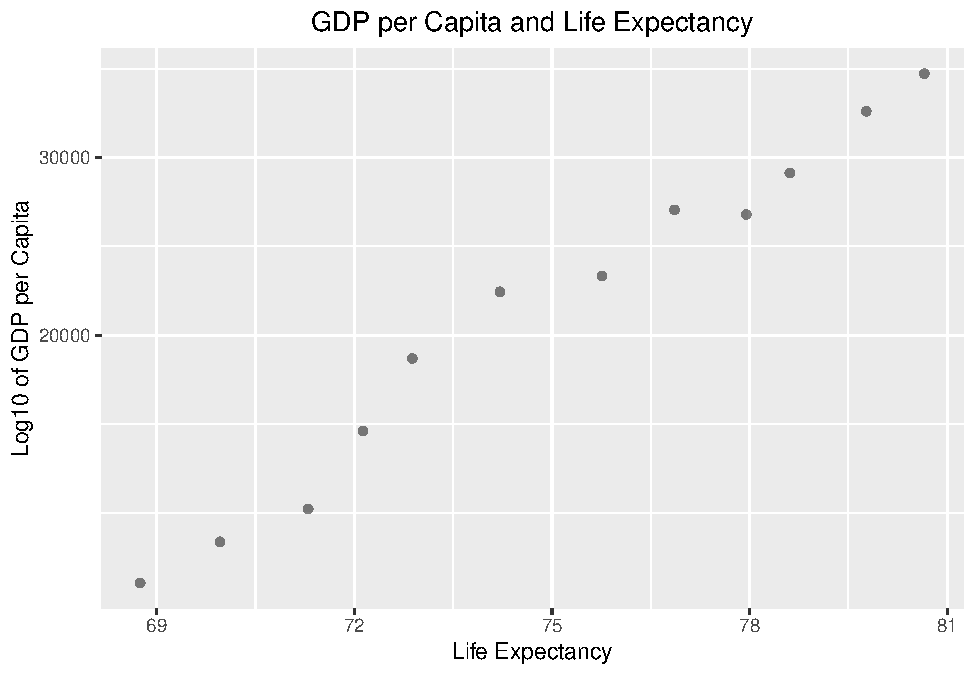
\includegraphics{hw02_files/figure-latex/Exercise 1.5-1.pdf}

\begin{center}\rule{0.5\linewidth}{\linethickness}\end{center}

\hypertarget{exercise-2}{%
\section{Exercise 2}\label{exercise-2}}

\textbf{Pick one categorical variable and one quantitative variable to
explore. Answer the following questions in whichever way you think is
appropriate, using dplyr:}

\textbf{What are possible values (or range, whichever is appropriate) of
each variable?}

\textbf{What values are typical? What's the spread? What's the
distribution? Etc., tailored to the variable at hand.}

\textbf{Feel free to use summary stats, tables, figures.}

\hypertarget{exploring-life-expectancy-variable}{%
\subsection{Exploring ``Life Expectancy''
Variable}\label{exploring-life-expectancy-variable}}

The range of life expectancy in this dataset is 23.6 years to 82.6
years.

\begin{Shaded}
\begin{Highlighting}[]
\KeywordTok{range}\NormalTok{(gapminder}\OperatorTok{$}\NormalTok{lifeExp)}
\end{Highlighting}
\end{Shaded}

\begin{verbatim}
## [1] 23.599 82.603
\end{verbatim}

\hypertarget{plot-of-the-average-life-expectancy-of-each-continent}{%
\paragraph{Plot of the average life expectancy of each
continent}\label{plot-of-the-average-life-expectancy-of-each-continent}}

\begin{Shaded}
\begin{Highlighting}[]
\NormalTok{gapminder }\OperatorTok
\StringTok{  }\KeywordTok{group_by}\NormalTok{(continent) }\OperatorTok
\StringTok{  }\KeywordTok{summarise}\NormalTok{(}\DataTypeTok{meanlifeExp =} \KeywordTok{mean}\NormalTok{(lifeExp)) }\OperatorTok
\StringTok{  }\KeywordTok{ggplot}\NormalTok{(}\KeywordTok{aes}\NormalTok{(continent, meanlifeExp)) }\OperatorTok{+}
\StringTok{  }\KeywordTok{geom_bar}\NormalTok{(}\DataTypeTok{stat =} \StringTok{"identity"}\NormalTok{) }\OperatorTok{+}
\StringTok{  }\KeywordTok{labs}\NormalTok{(}\DataTypeTok{title =} \StringTok{"Mean Life Expectancy by Continent"}\NormalTok{, }
       \DataTypeTok{x =} \StringTok{"Continent"}\NormalTok{, }
       \DataTypeTok{y =} \StringTok{"Mean Life Expectancy"}\NormalTok{) }\OperatorTok{+}
\StringTok{  }\KeywordTok{theme}\NormalTok{(}\DataTypeTok{plot.title =} \KeywordTok{element_text}\NormalTok{(}\DataTypeTok{hjust =} \FloatTok{0.5}\NormalTok{))}
\end{Highlighting}
\end{Shaded}

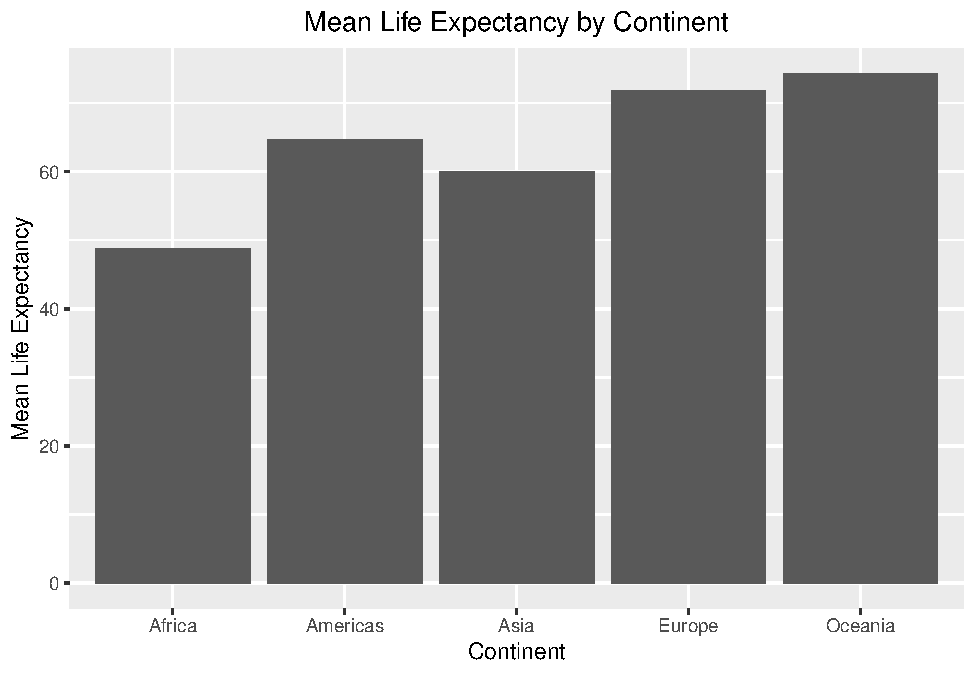
\includegraphics{hw02_files/figure-latex/Exercise 2 lifeExp2-1.pdf}

\hypertarget{exploring-continent-and-country-variables}{%
\subsection{Exploring ``Continent'' and ``Country''
Variables}\label{exploring-continent-and-country-variables}}

\emph{The following shows the number of countries from each continent in
this the ``gapminder'' dataset.}

\begin{Shaded}
\begin{Highlighting}[]
\NormalTok{gapminder }\OperatorTok
\StringTok{  }\KeywordTok{group_by}\NormalTok{(continent) }\OperatorTok
\StringTok{  }\KeywordTok{summarize}\NormalTok{(}\DataTypeTok{n_of_countries =} \KeywordTok{n_distinct}\NormalTok{(country)) }\OperatorTok
\StringTok{  }\NormalTok{knitr}\OperatorTok{::}\KeywordTok{kable}\NormalTok{()}
\end{Highlighting}
\end{Shaded}

\begin{longtable}[]{@{}lr@{}}
\toprule
continent & n\_of\_countries\tabularnewline
\midrule
\endhead
Africa & 52\tabularnewline
Americas & 25\tabularnewline
Asia & 33\tabularnewline
Europe & 30\tabularnewline
Oceania & 2\tabularnewline
\bottomrule
\end{longtable}

\begin{Shaded}
\begin{Highlighting}[]
\NormalTok{gapminder }\OperatorTok
\StringTok{  }\KeywordTok{group_by}\NormalTok{(continent) }\OperatorTok
\StringTok{  }\KeywordTok{summarize}\NormalTok{(}\DataTypeTok{n_countries =} \KeywordTok{n_distinct}\NormalTok{(country)) }\OperatorTok
\StringTok{  }\KeywordTok{ggplot}\NormalTok{(}\KeywordTok{aes}\NormalTok{(continent, n_countries)) }\OperatorTok{+}
\StringTok{  }\KeywordTok{geom_bar}\NormalTok{(}\DataTypeTok{stat =} \StringTok{"identity"}\NormalTok{) }\OperatorTok{+}
\StringTok{  }\KeywordTok{labs}\NormalTok{(}\DataTypeTok{title =} \StringTok{"Number of Countries from Each Continent"}\NormalTok{, }\DataTypeTok{x =} \StringTok{"Continent"}\NormalTok{, }\DataTypeTok{y =} \StringTok{"Number of Countries"}\NormalTok{) }\OperatorTok{+}
\StringTok{  }\KeywordTok{theme}\NormalTok{(}\DataTypeTok{plot.title =} \KeywordTok{element_text}\NormalTok{(}\DataTypeTok{hjust =} \FloatTok{0.5}\NormalTok{))}
\end{Highlighting}
\end{Shaded}

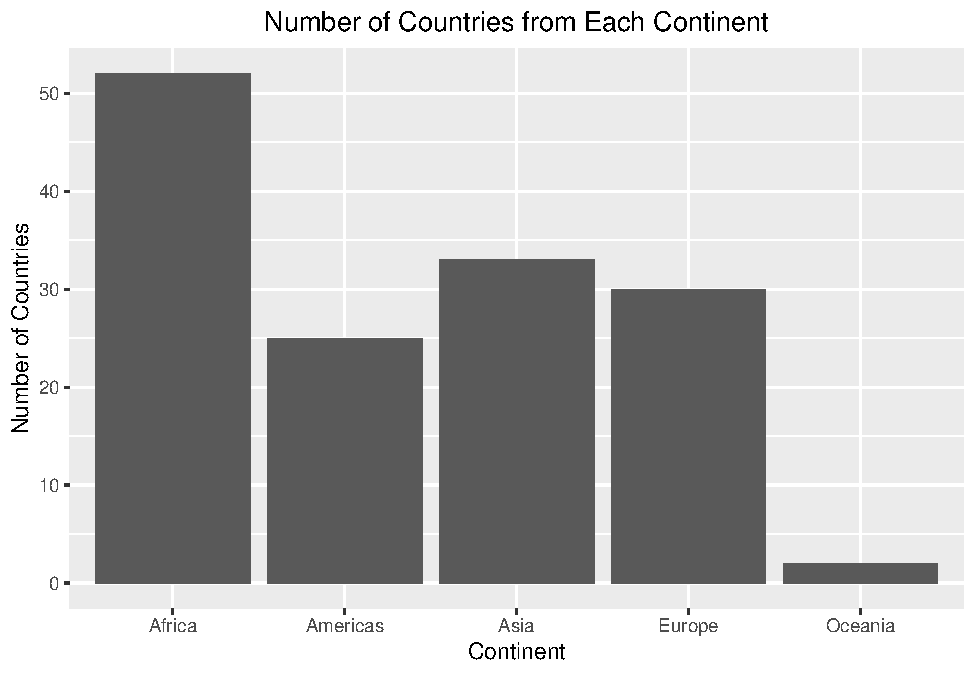
\includegraphics{hw02_files/figure-latex/Exercise 2, plot continent and country-1.pdf}

\begin{center}\rule{0.5\linewidth}{\linethickness}\end{center}

\hypertarget{exercise-3}{%
\section{Exercise 3}\label{exercise-3}}

\textbf{Make two plots that have some value to them. That is, plots that
someone might actually consider making for an analysis. Just don't make
the same plots we made in class -- feel free to use a data set from the
datasets R package if you wish.}

\textbf{A scatterplot of two quantitative variables.} \textbf{One other
plot besides a scatterplot.} \textbf{You don't have to use all the data
in every plot! It's fine to filter down to one country or a small
handful of countries.}

\hypertarget{scatterplot-made-using-orange-dataset}{%
\subsection{Scatterplot made using ``Orange''
dataset}\label{scatterplot-made-using-orange-dataset}}

\hypertarget{information-about-orange-dataset}{%
\subsubsection{Information about ``Orange''
dataset}\label{information-about-orange-dataset}}

\emph{From
\url{https://stat.ethz.ch/R-manual/R-devel/library/datasets/html/Orange.html}}

\emph{"Tree}

\emph{an ordered factor indicating the tree on which the measurement is
made. The ordering is according to increasing maximum diameter.}

\emph{age}

\emph{a numeric vector giving the age of the tree (days since
1968/12/31)}

\emph{circumference}

\emph{a numeric vector of trunk circumferences (mm). This is probably
``circumference at breast height'', a standard measurement in
forestry."}

\hypertarget{plot-of-the-age-and-the-circumference-of-orange-trees}{%
\subsubsection{Plot of the age and the circumference of orange
trees}\label{plot-of-the-age-and-the-circumference-of-orange-trees}}

\begin{Shaded}
\begin{Highlighting}[]
\KeywordTok{data}\NormalTok{(Orange)}
\NormalTok{Orange }\OperatorTok
\StringTok{  }\KeywordTok{ggplot}\NormalTok{(}\KeywordTok{aes}\NormalTok{(age, circumference)) }\OperatorTok{+}
\StringTok{  }\KeywordTok{geom_point}\NormalTok{(}\DataTypeTok{alpha =} \FloatTok{0.4}\NormalTok{) }\OperatorTok{+}
\StringTok{  }\KeywordTok{labs}\NormalTok{(}\DataTypeTok{title =} \StringTok{"Circumference by Age"}\NormalTok{, }\DataTypeTok{x =} \StringTok{"Age"}\NormalTok{, }\DataTypeTok{y =} \StringTok{"Circumference (mm)"}\NormalTok{) }\OperatorTok{+}
\StringTok{  }\KeywordTok{theme}\NormalTok{(}\DataTypeTok{plot.title =} \KeywordTok{element_text}\NormalTok{(}\DataTypeTok{hjust =} \FloatTok{0.5}\NormalTok{))}
\end{Highlighting}
\end{Shaded}

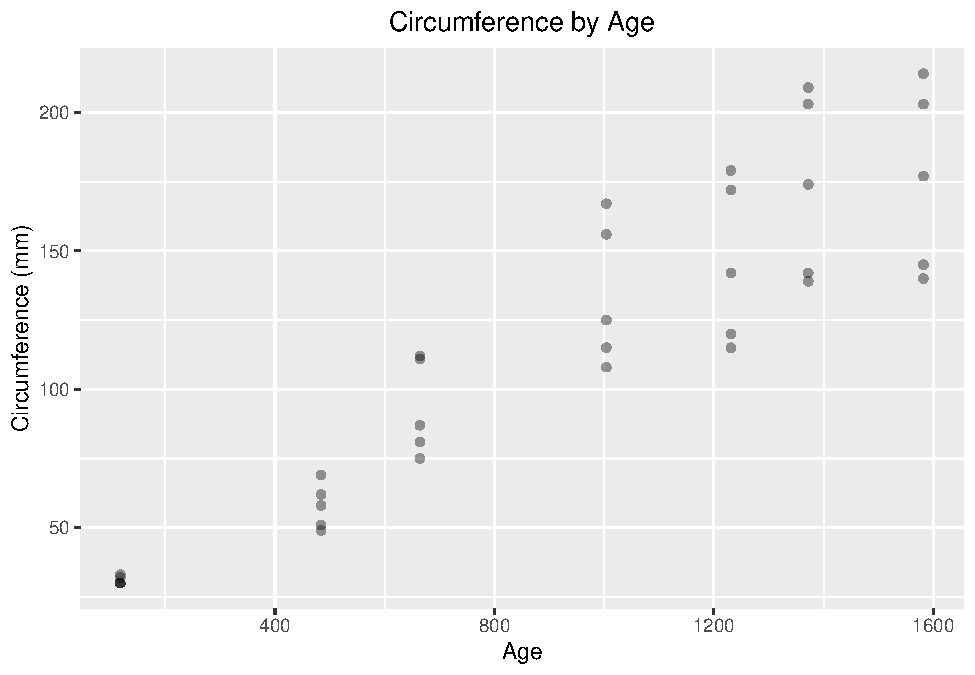
\includegraphics{hw02_files/figure-latex/load Orange dataset, scatter Orange-1.pdf}

\hypertarget{boxplot-made-using-the-sleep-dataset}{%
\subsection{Boxplot made using the ``sleep''
dataset}\label{boxplot-made-using-the-sleep-dataset}}

\hypertarget{information-about-sleep-dataset}{%
\subsubsection{Information about ``sleep''
dataset}\label{information-about-sleep-dataset}}

\emph{The following is an exploration of the ``sleep'' dataset.}
\emph{From:
\url{https://stat.ethz.ch/R-manual/R-devel/library/datasets/html/sleep.html}}

\emph{``Data which show the effect of two soporific drugs (increase in
hours of sleep compared to control) on 10 patients.''}

\begin{longtable}[]{@{}ll@{}}
\toprule
Variables & Explanation\tabularnewline
\midrule
\endhead
extra & ``increase in hours of sleep''\tabularnewline
group & ``drug given''\tabularnewline
ID & ``patient ID''\tabularnewline
\bottomrule
\end{longtable}

\hypertarget{boxplot-of-increase-in-sleep}{%
\subsubsection{Boxplot of Increase in
Sleep}\label{boxplot-of-increase-in-sleep}}

\begin{Shaded}
\begin{Highlighting}[]
\KeywordTok{data}\NormalTok{(sleep)}
\NormalTok{sleep }\OperatorTok
\StringTok{  }\KeywordTok{group_by}\NormalTok{(group) }\OperatorTok
\StringTok{  }\KeywordTok{ggplot}\NormalTok{(}\KeywordTok{aes}\NormalTok{(group, extra)) }\OperatorTok{+}
\StringTok{  }\KeywordTok{geom_boxplot}\NormalTok{() }\OperatorTok{+}
\StringTok{  }\KeywordTok{labs}\NormalTok{(}\DataTypeTok{title =} \StringTok{"Increase in Sleep for Each Drug Group"}\NormalTok{, }\DataTypeTok{x =} \StringTok{"Type of Drug Given"}\NormalTok{, }\DataTypeTok{y =} \StringTok{"Increase in Sleep (hours)"}\NormalTok{) }\OperatorTok{+}
\StringTok{  }\KeywordTok{theme}\NormalTok{(}\DataTypeTok{plot.title =} \KeywordTok{element_text}\NormalTok{(}\DataTypeTok{hjust =} \FloatTok{0.5}\NormalTok{))}
\end{Highlighting}
\end{Shaded}

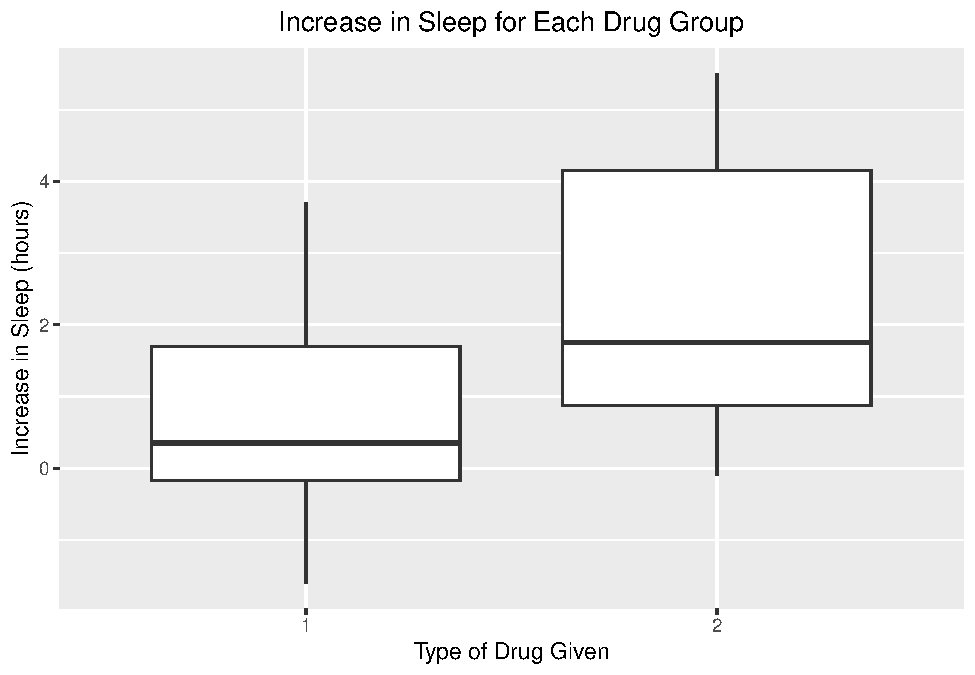
\includegraphics{hw02_files/figure-latex/load sleep and boxplot of sleep-1.pdf}


\end{document}
